\subsection{Allgemeine Datenanalyse}
\label{subsec:Datenanalyse}
Die Datenanalyse ist ein, wenn nicht sogar der Wichtigste schritt im Data Science Bereich \cite{Agarwal.05.10.2018}. Dabei sollen die Daten ergründet und verstanden werden. Dieser Schritt soll nicht nur ein Verständnis für die vorliegenden Daten schaffen, sondern auch \emph{outlier} erfassen. Meist wird auch versucht innerhalb der Datenanalyse zusammenhänge zu der Zielvariable zu finden. Dies setzt jedoch voraus, dass eine Zielvariable vorhanden ist. In dem vorliegenden Fall existiert keine Zielvariable, da nicht bekannt ist welche Hotels mit welchen Hotels ähnlich sind. Aufgrund dessen, dass keine Zielvariable vorhanden ist, wird die folgende Datenanalyse lediglich dazu genutzt um die Daten besser zu verstehen. Zudem soll festgestellt werden, welche Daten wie als Features verwendet werden können.
\newline
\newline
Für die Datenanalyse soll die Python-Bibliothek \emph{Seaborn} benutzt werden. Die \emph{Seaborn}-Bibliothek stellt ein leistungsstarkes Werkzeug dar, das speziell für die Erstellung von statistischen Grafiken in Python entwickelt wurde \cite{Melanie.2023}. Das Hauptziel besteht darin, die verschiedenen Verteilungen der Features auf anschauliche Weise darzustellen, um einen umfassenden Überblick über die zugrunde liegenden Daten zu ermöglichen. Durch die Nutzung der Funktionalitäten von \emph{Seaborn} wird eine effiziente und ästhetisch ansprechende Visualisierung erreicht, die es ermöglicht, Muster, Ausreißer oder Trends in den Daten leichter zu identifizieren.

\subsubsection{Region Features}
Zuallererst soll ein grober Überblick über die Städte der Hotels innerhalb der Datenbank erstellt werden. Dazu wird innerhalb des Datensatzes nach der Stadt um die Anzahl der Hotels einer Stadt zu ermitteln.

\newpage

\begin{figure}[h]
    \centering
    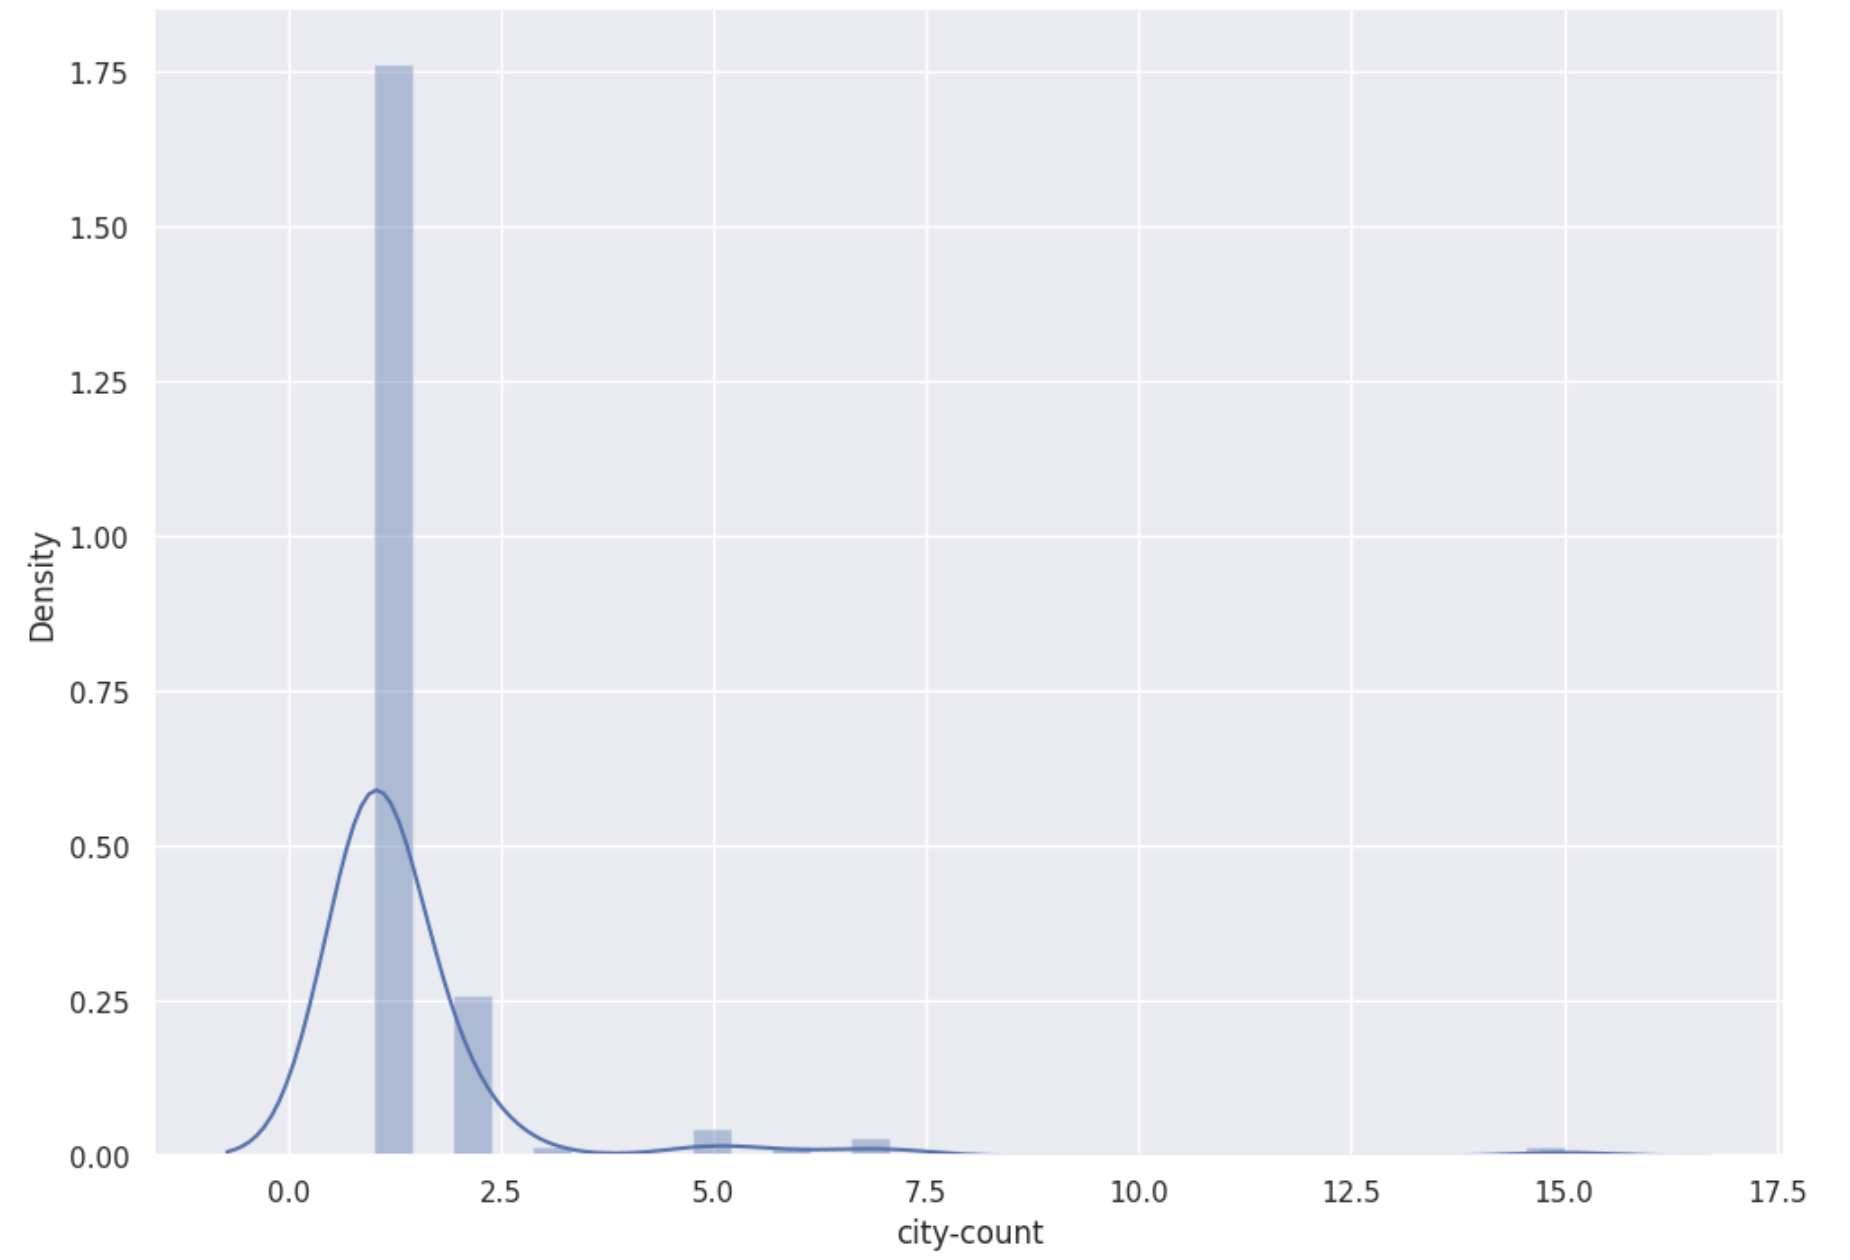
\includegraphics[width=1\textwidth, center]{verteilung_city.png}
    \caption[Verteilung der Städte]{Verteilung der Städte}
    \label{img:verteilung_city}
\end{figure}

Die Analyse der Abbildung \ref{img:verteilung_city} offenbart, dass die überwiegende Mehrheit der in der Datenbank erfassten Städte lediglich über ein einziges Hotel verfügt, welches happyhotel in Anspruch nimmt. Zugleich verdeutlicht die Abbildung \ref{img:verteilung_city}, dass es lediglich einen geringen Anteil von Städten gibt, in denen fünf oder mehr Hotels registriert sind. Dies ist etwas problematisch, da das Feature \emph{City} zu unausgewogen ist und so nicht mit in das Modell gegeben werden kann. Es muss also in einer anderen Form verwendet werden.
\newline
\newline
Momentan werden, wie in der Abbildung \ref{img:all_Features_2} gezeigt, die Stadt und die Region als zwei separate Features aufgelistet. Die Idee ist es nun die zwei Features zu verschmelzen und die Hotels in Regionen aufzuteilen um mehr Informationen zu erhalten. Anstatt also Region und Stadt separat zu haben soll es ein Feature Region geben, welches wie folgt aufgebaut ist: 

\begin{itemize}
    \item Befindet sich innerhalb einer Stadt Fünf oder mehr Hotels, so wird die Stadt ohne jegliche Modifikation als Region genommen.
    \item Befindet sich innerhalb einer Stadt weniger als Fünf Hotels, so setzt sich die Region aus der ursprünglichen Region, also dem Bundesland und der Größe der Stadt zusammen nach dem Schema: {Region}-{Größe}
\end{itemize}

Für die Idee muss zunächst ermittelt werden, in welchen Städte sich Fünf oder mehr Hotels befinden. Auch diese Information kann wie folgt Visualisiert werden:

\begin{figure}[h]
    \centering
    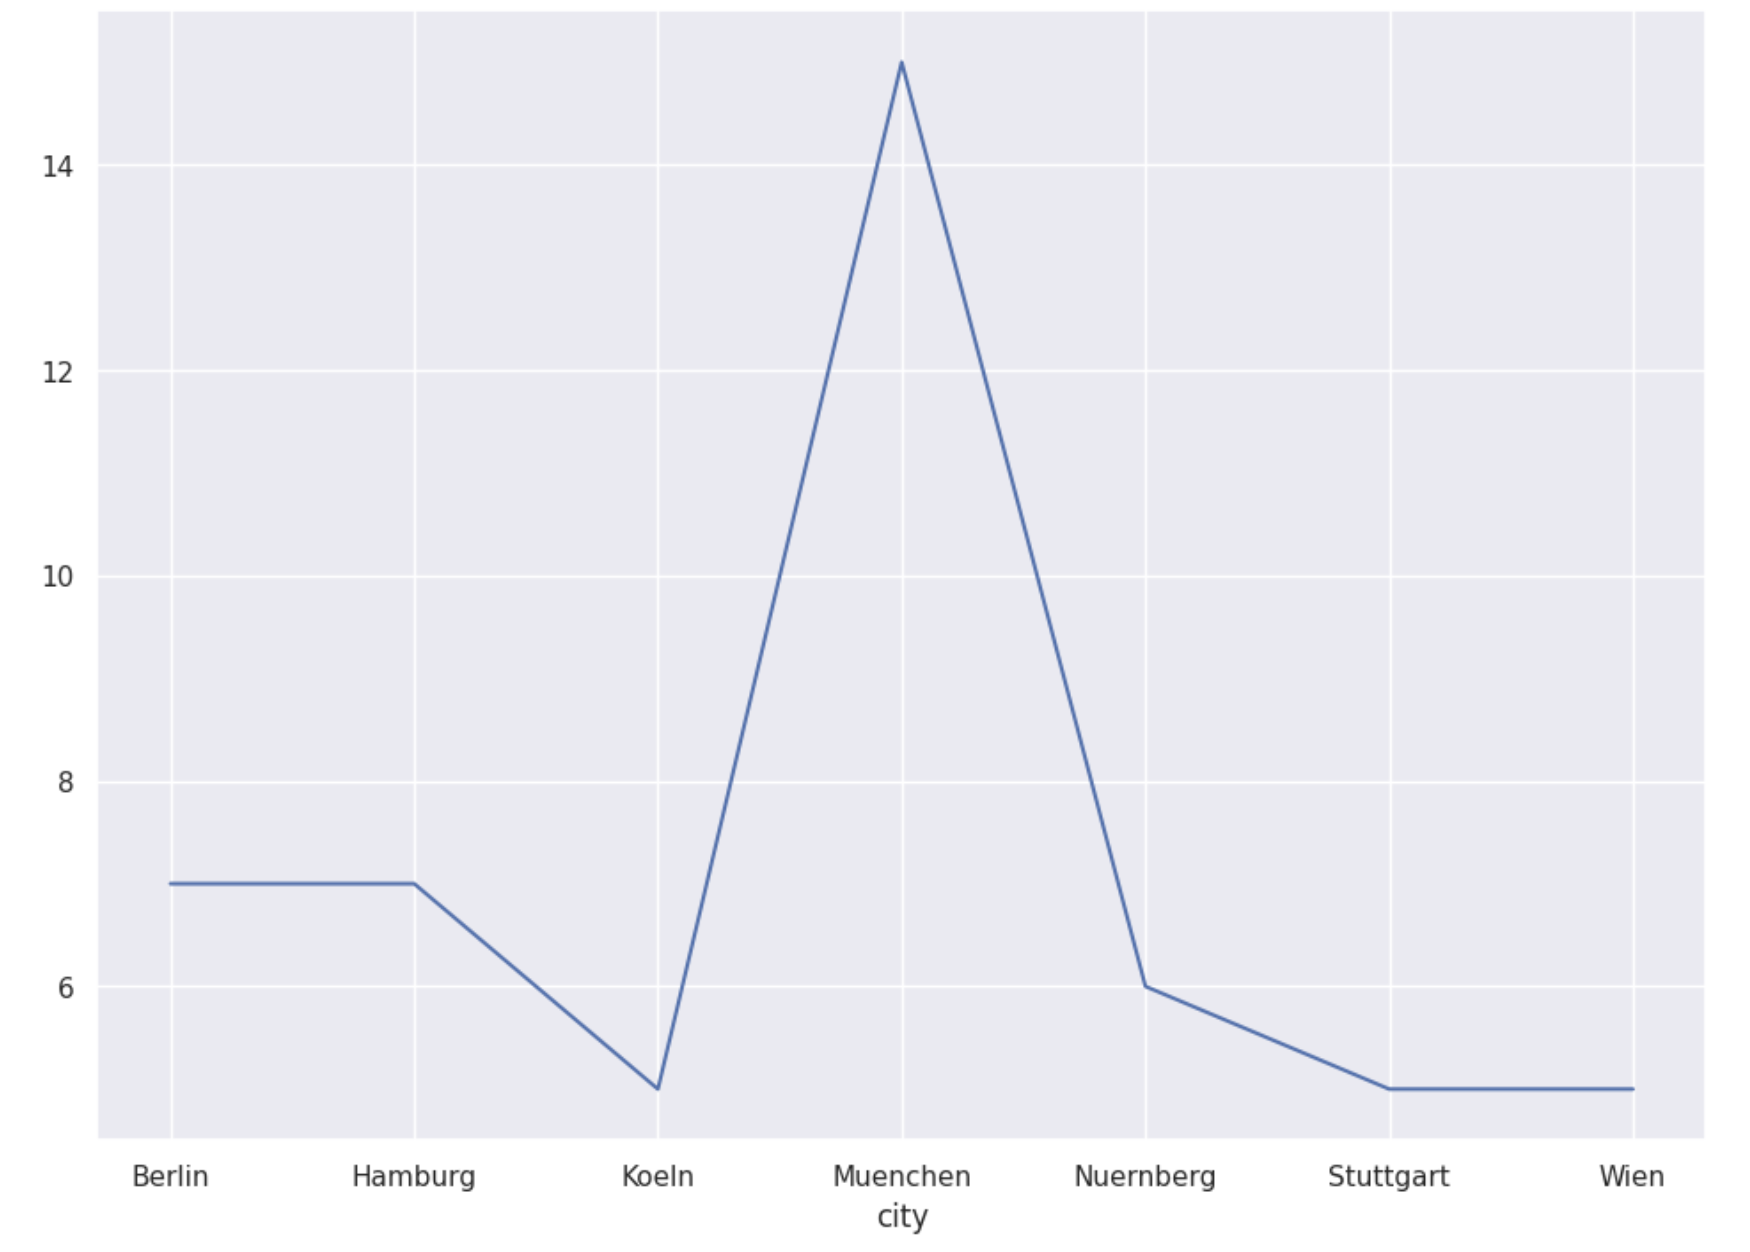
\includegraphics[width=1\textwidth, center]{city_five_or_more.png}
    \caption[Städte mit Fünf oder mehr Hotels]{Städte mit Fünf oder mehr Hotels}
    \label{img:city_five_or_more}
\end{figure}

Ganz klar zu erkennen ist, dass die Sieben Städte Berlin, Hamburg, Köln, München, Nürnberg, Stuttgart, und Wien die Städte sind, in denen Fünf oder mehr Hotels vorhanden sind. Die aufgelisteten Städte können dementsprechend so übernommen werden und für alle anderen wird die Regel von oben angewandt.
\newline
Nach der Umformulierung von Region und Stadt sieht der Datensatz wie folgt aus:

\begin{figure}[h]
    \centering
    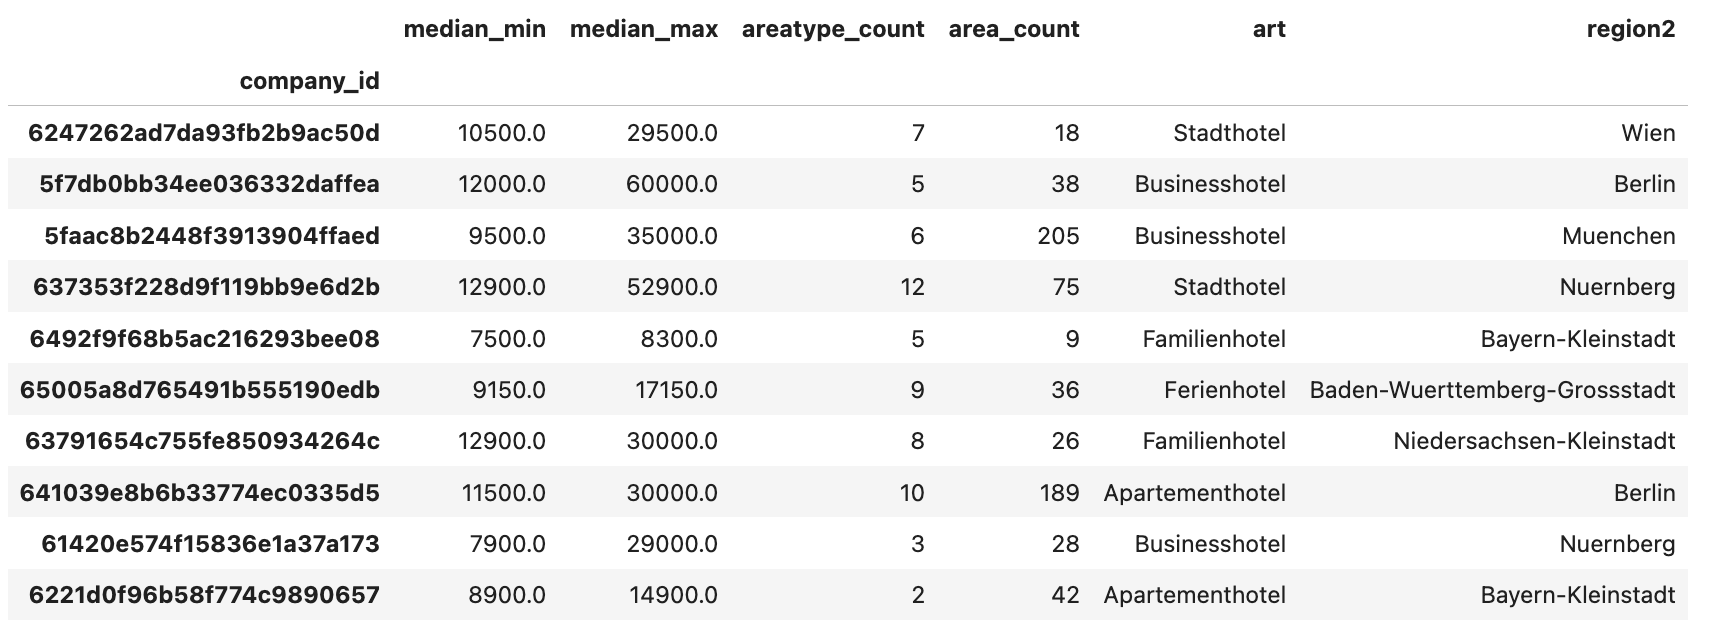
\includegraphics[width=1\textwidth, center]{all_features_3.png}
    \caption[Datensatz nach der Umformulierung]{Datensatz nach der Umformulierung}
    \label{img:all_features_3}
\end{figure}

Auch hier soll wieder die Verteilung visualisiert werden

\begin{figure}[h]
    \centering
    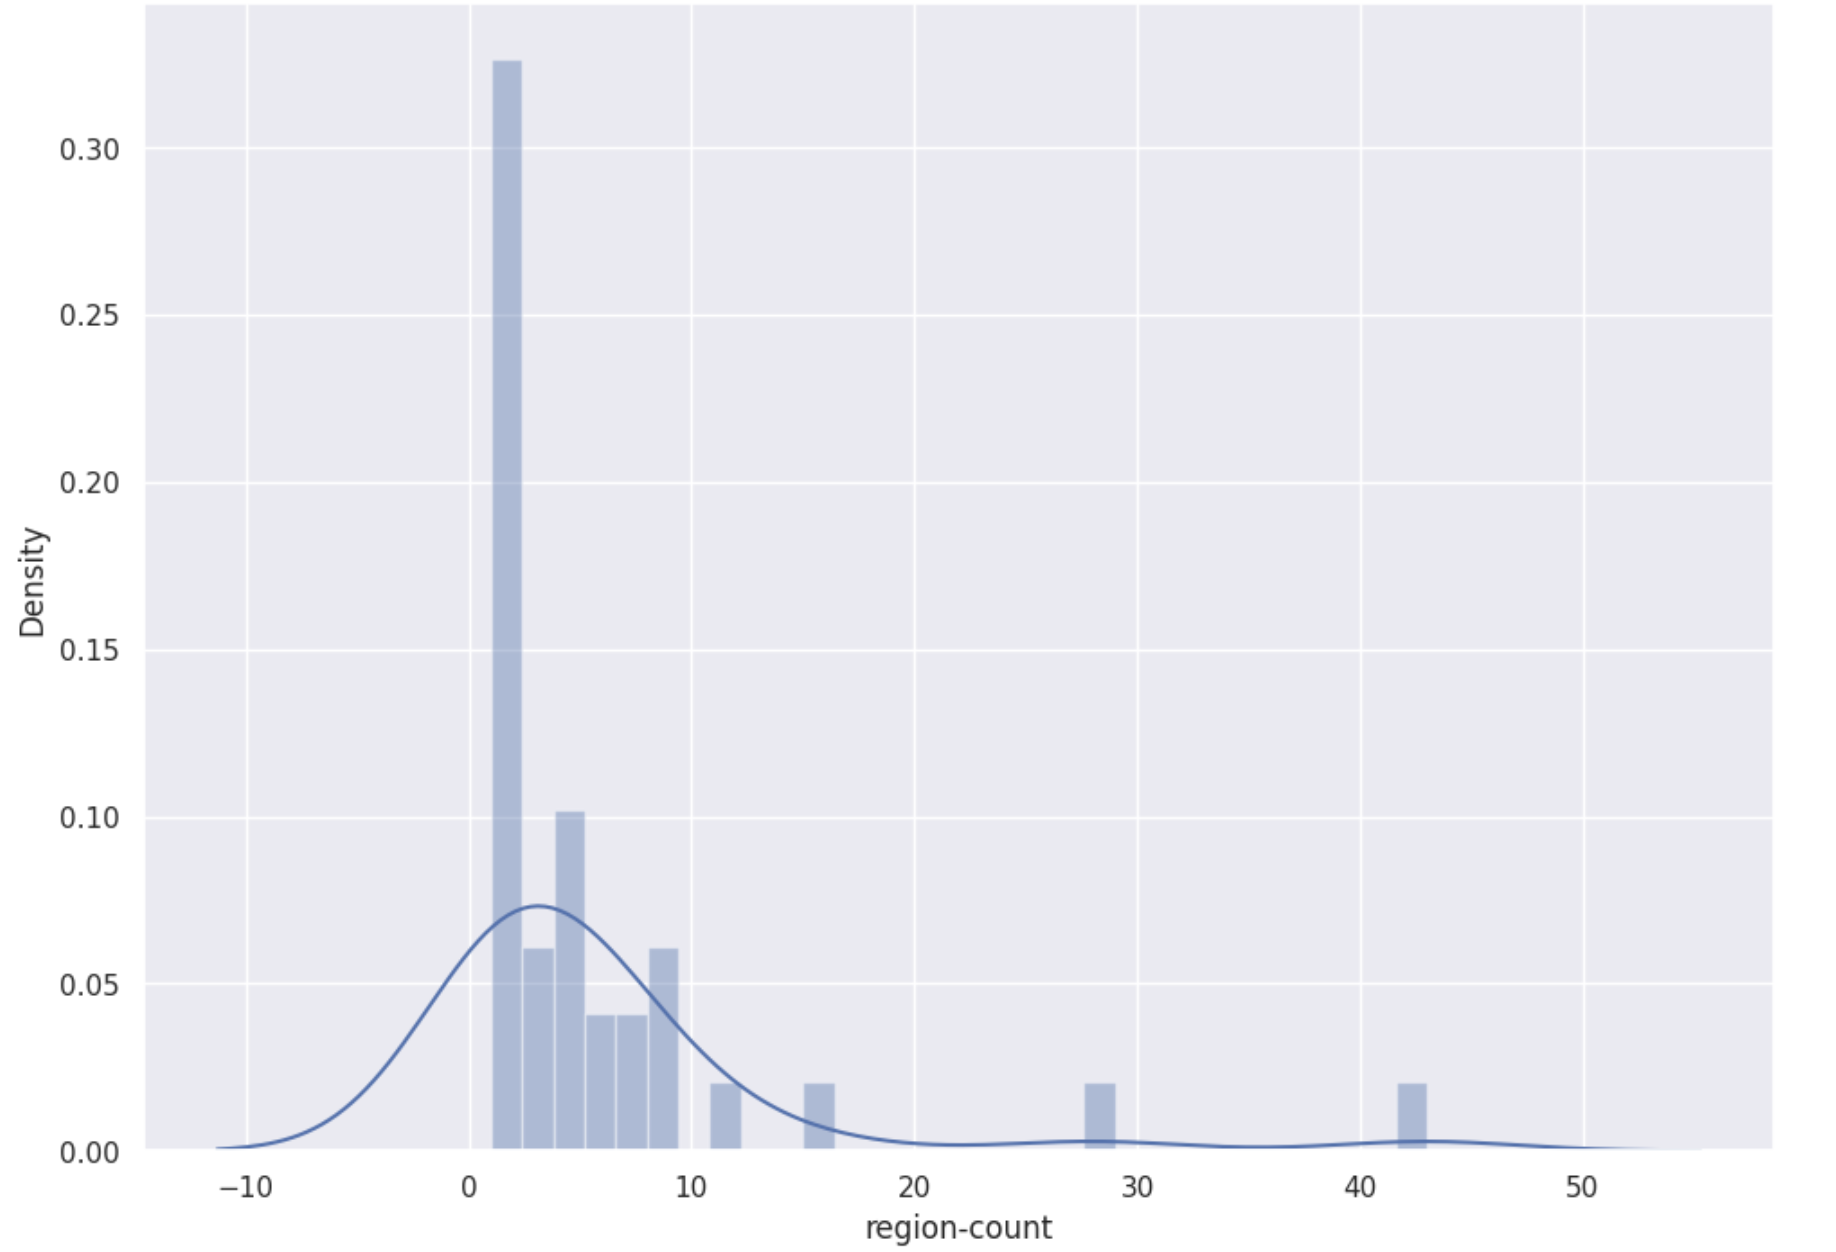
\includegraphics[width=1\textwidth, center]{verteilung_region2.png}
    \caption[Verteilung des neuen Features \emph{region2}]{Verteilung des neuen Features \emph{region2}}
    \label{img:verteilung_region_2}
\end{figure}

Es zeigt sich, dass noch immer ein großer Anteil des Datensatzes niedrigeren Bereich sich befindet, jedoch konnte mit der Modifikation ein bisschen mehr Varianz in die Daten gebracht werden.

\subsubsection{Preis Features}
Als nächstes sollen die Preis Features, namentlich betitelt mit \emph{median\_min} und \emph{median\_max}, erkundet und visualisiert werden. Hierzu soll wie auch bei der Region zunächst die Verteilung betrachtet werden:
\newpage
\begin{figure}[h]
    \centering
    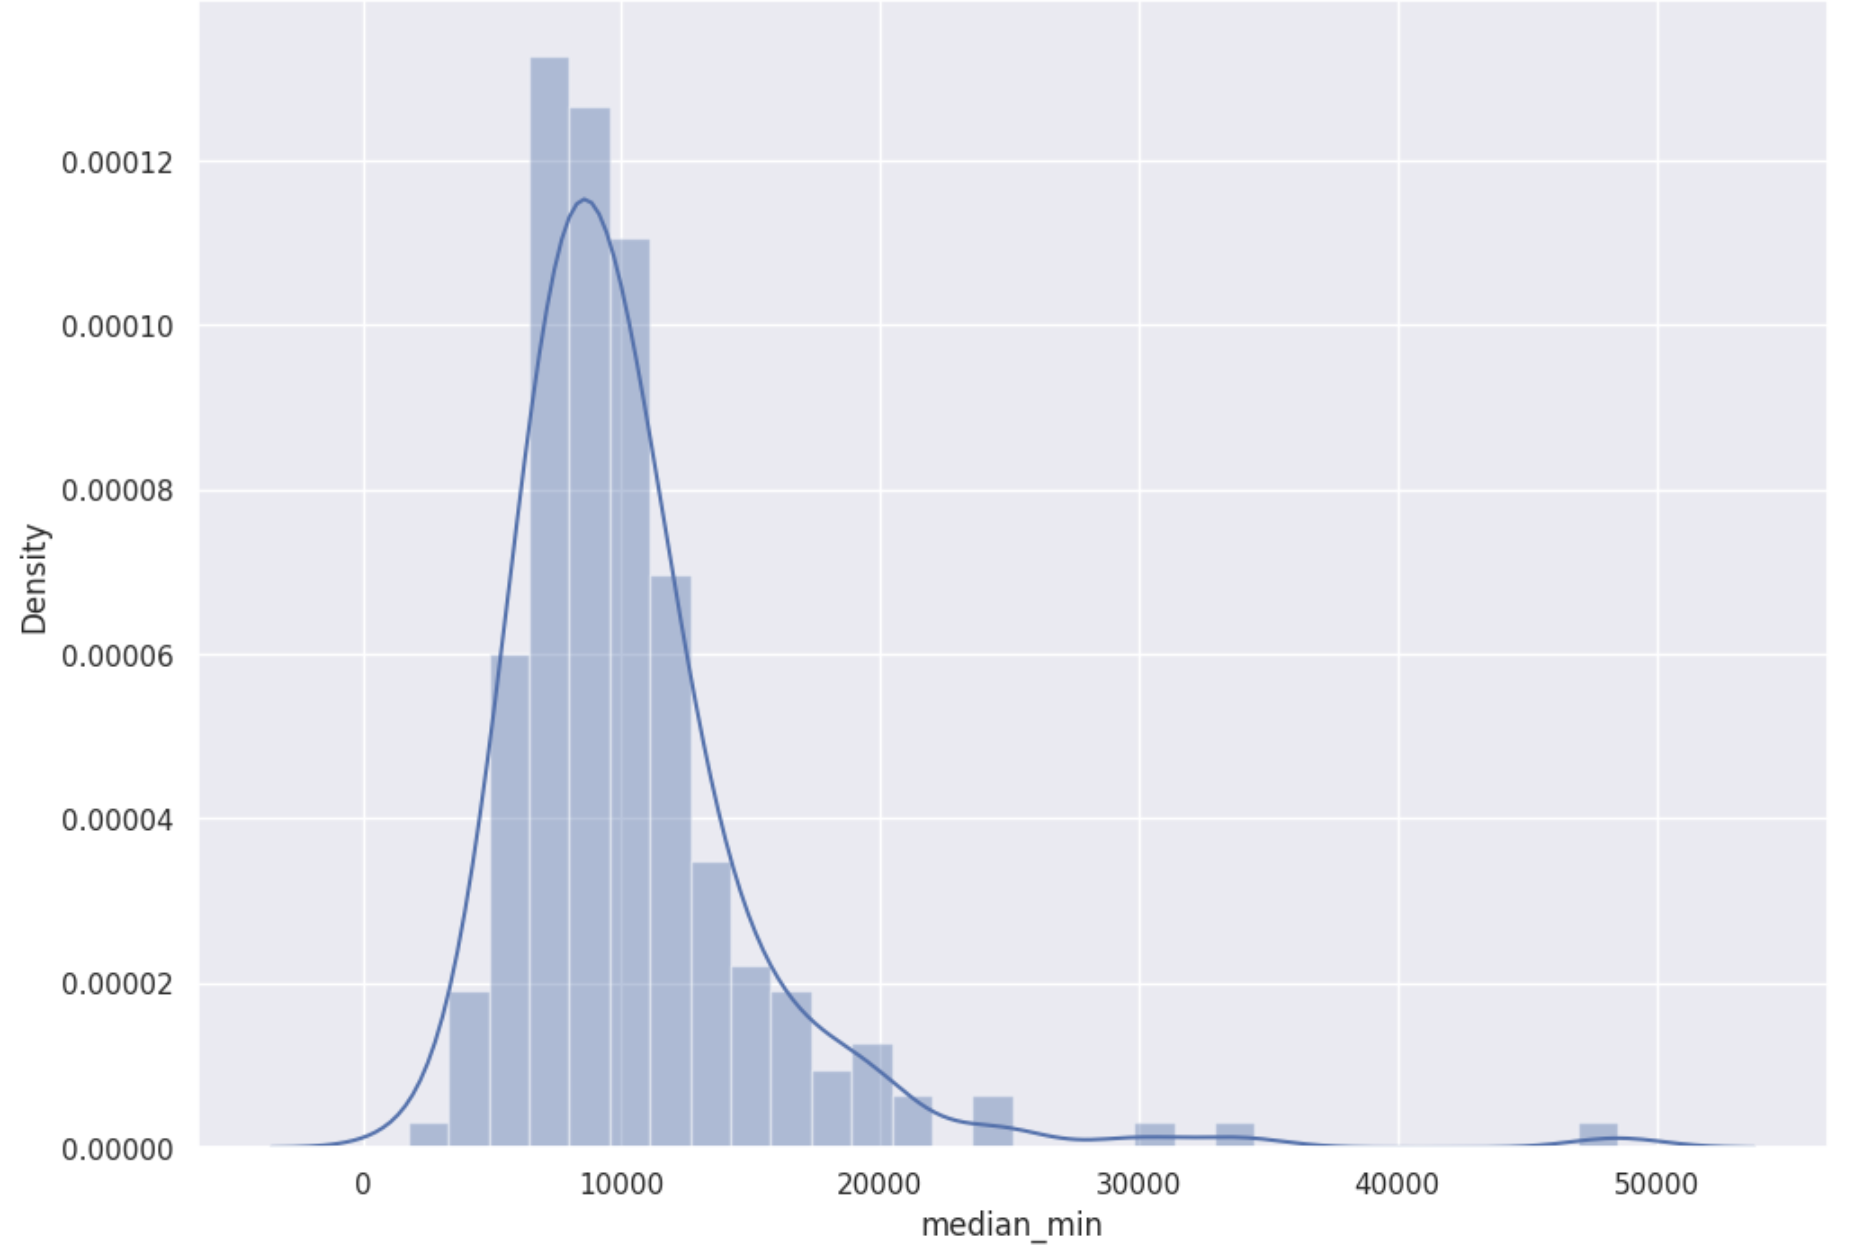
\includegraphics[width=1\textwidth, center]{verteilung_min.png}
    \caption[Verteilung von dem Preis Features \emph{median\_min}]{Verteilung von dem Preis Features \emph{median\_min}}
    \label{img:verteilung_min}
\end{figure}

Abbildung \ref{img:verteilung_min} zeigt, dass das Feature \emph{median\_min} eine Normalverteilung mit ein paar outlier aufweist. Eine Normalverteilung  sagt aus, dass die Verteilung mehr Daten um den Mittelwert herum aufweist. Die Datenverteilung nimmt ab, wenn sich vom Zentrum entfernt wird. Die resultierende Kurve ist symmetrisch zum Mittelwert und bildet eine glockenförmige Verteilung \cite{Shrishty.05.08.2021}.
\newline
\newline
Eine weitere interessante Information die noch aus dem Feature \emph{median\_min} gelesen werden kann, ist der Durchschnittliche Wert Region. Dazu soll der Datensatz nach der Region gruppiert werden und den Durchschnittlichen Wert ermittelt werden.
\newpage
\begin{figure}[h]
    \centering
    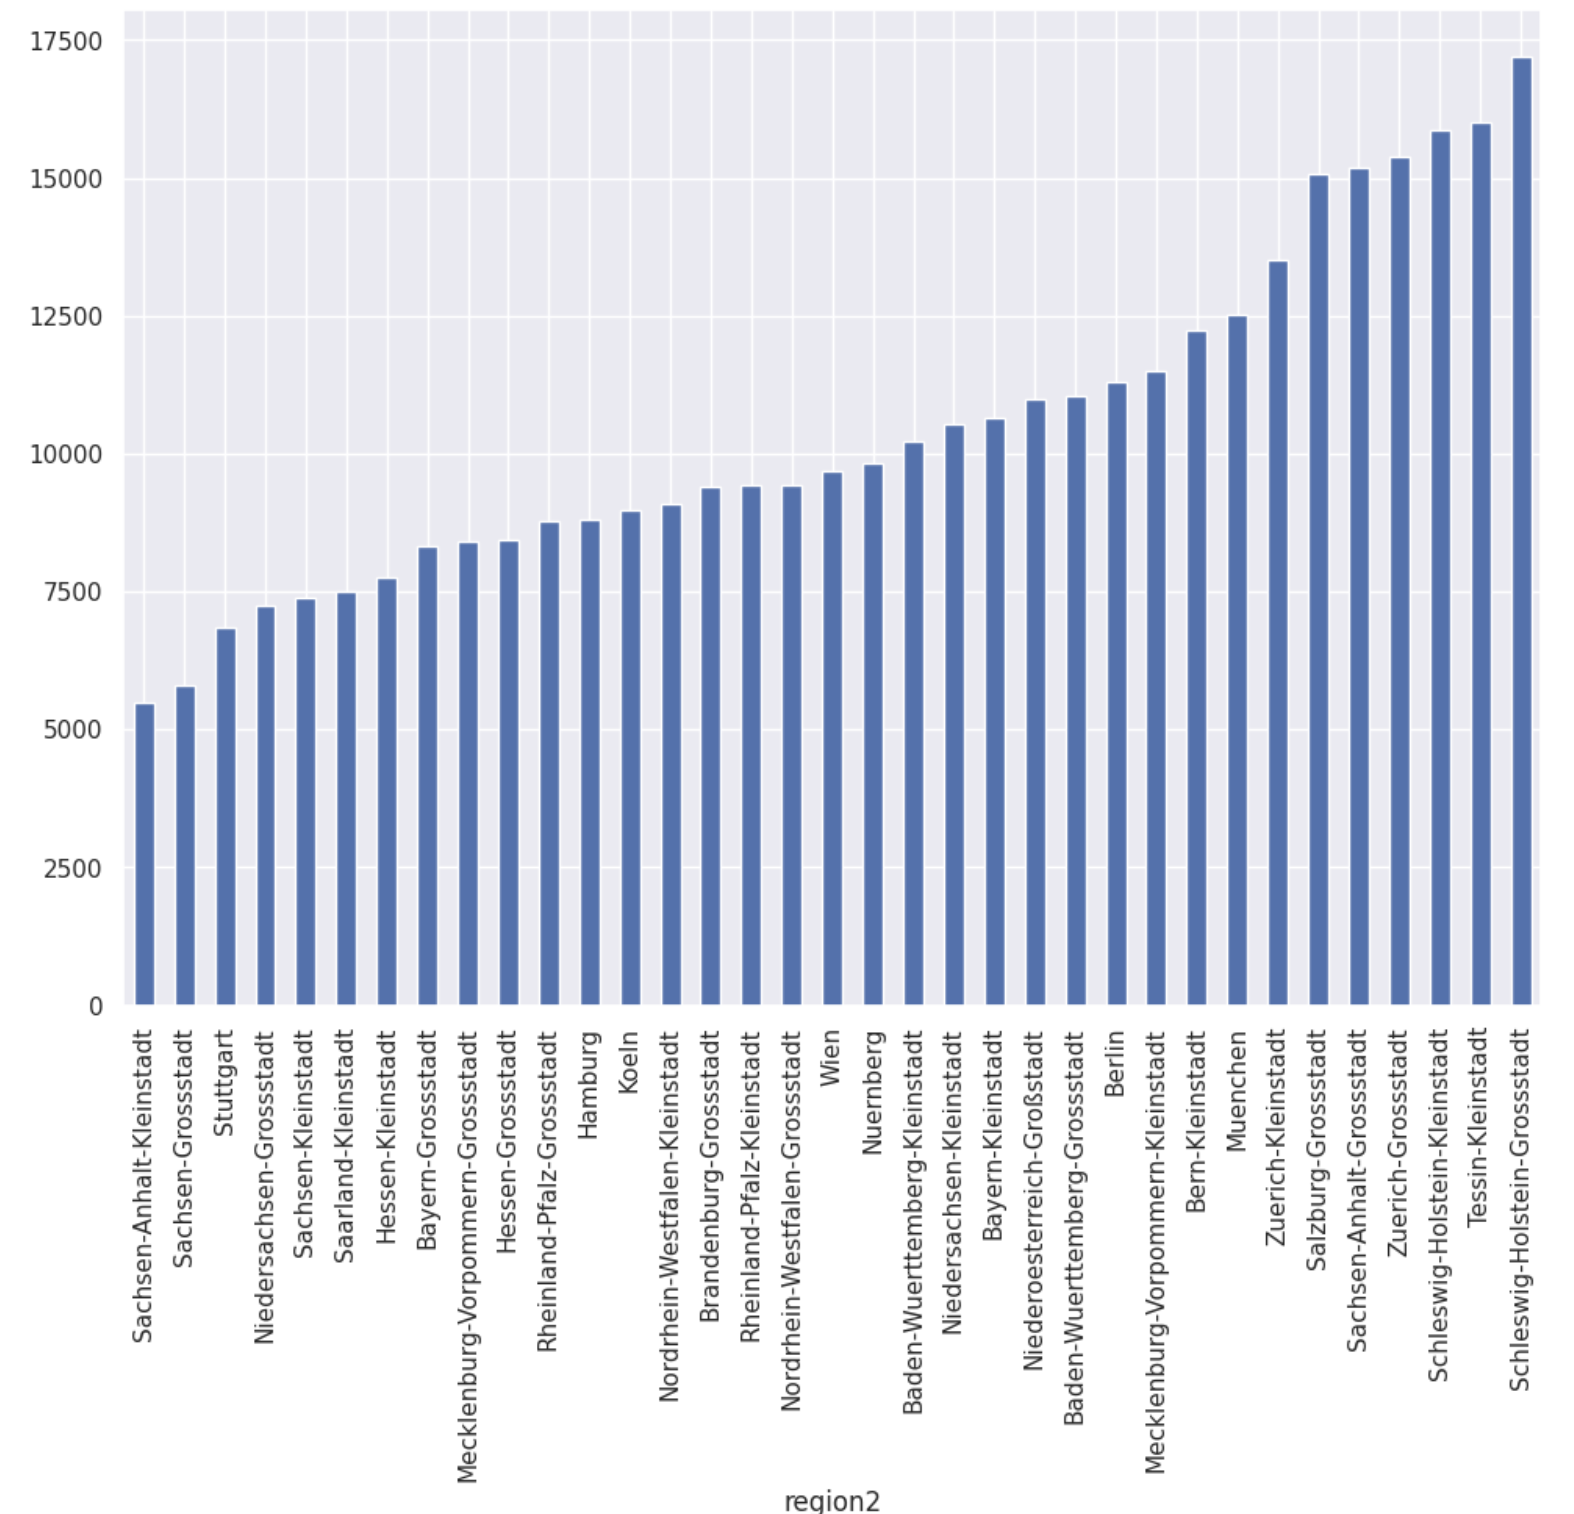
\includegraphics[width=0.6\textwidth, center]{avg_min_city.png}
    \caption[Durchschnittlicher minimal Preis pro Region]{Durchschnittlicher minimal Preis pro Region}
    \label{img:avg_min_city}
\end{figure}

Die Erkenntnis die aus der Abbildung \ref{img:avg_min_city} genommen werden kann, ist die, dass es einen deutlichen unterschied macht, in welcher Region das Hotel liegt wenn auf den Minimalen Median Preis des Hotel geschaut wird. Das gleich kann auch mit dem Maximalen Median Preis eines Hotels gemacht werden. Auch hier soll sich zunächst die Verteilung visualisiert werden:

\begin{figure}[h]
    \centering
    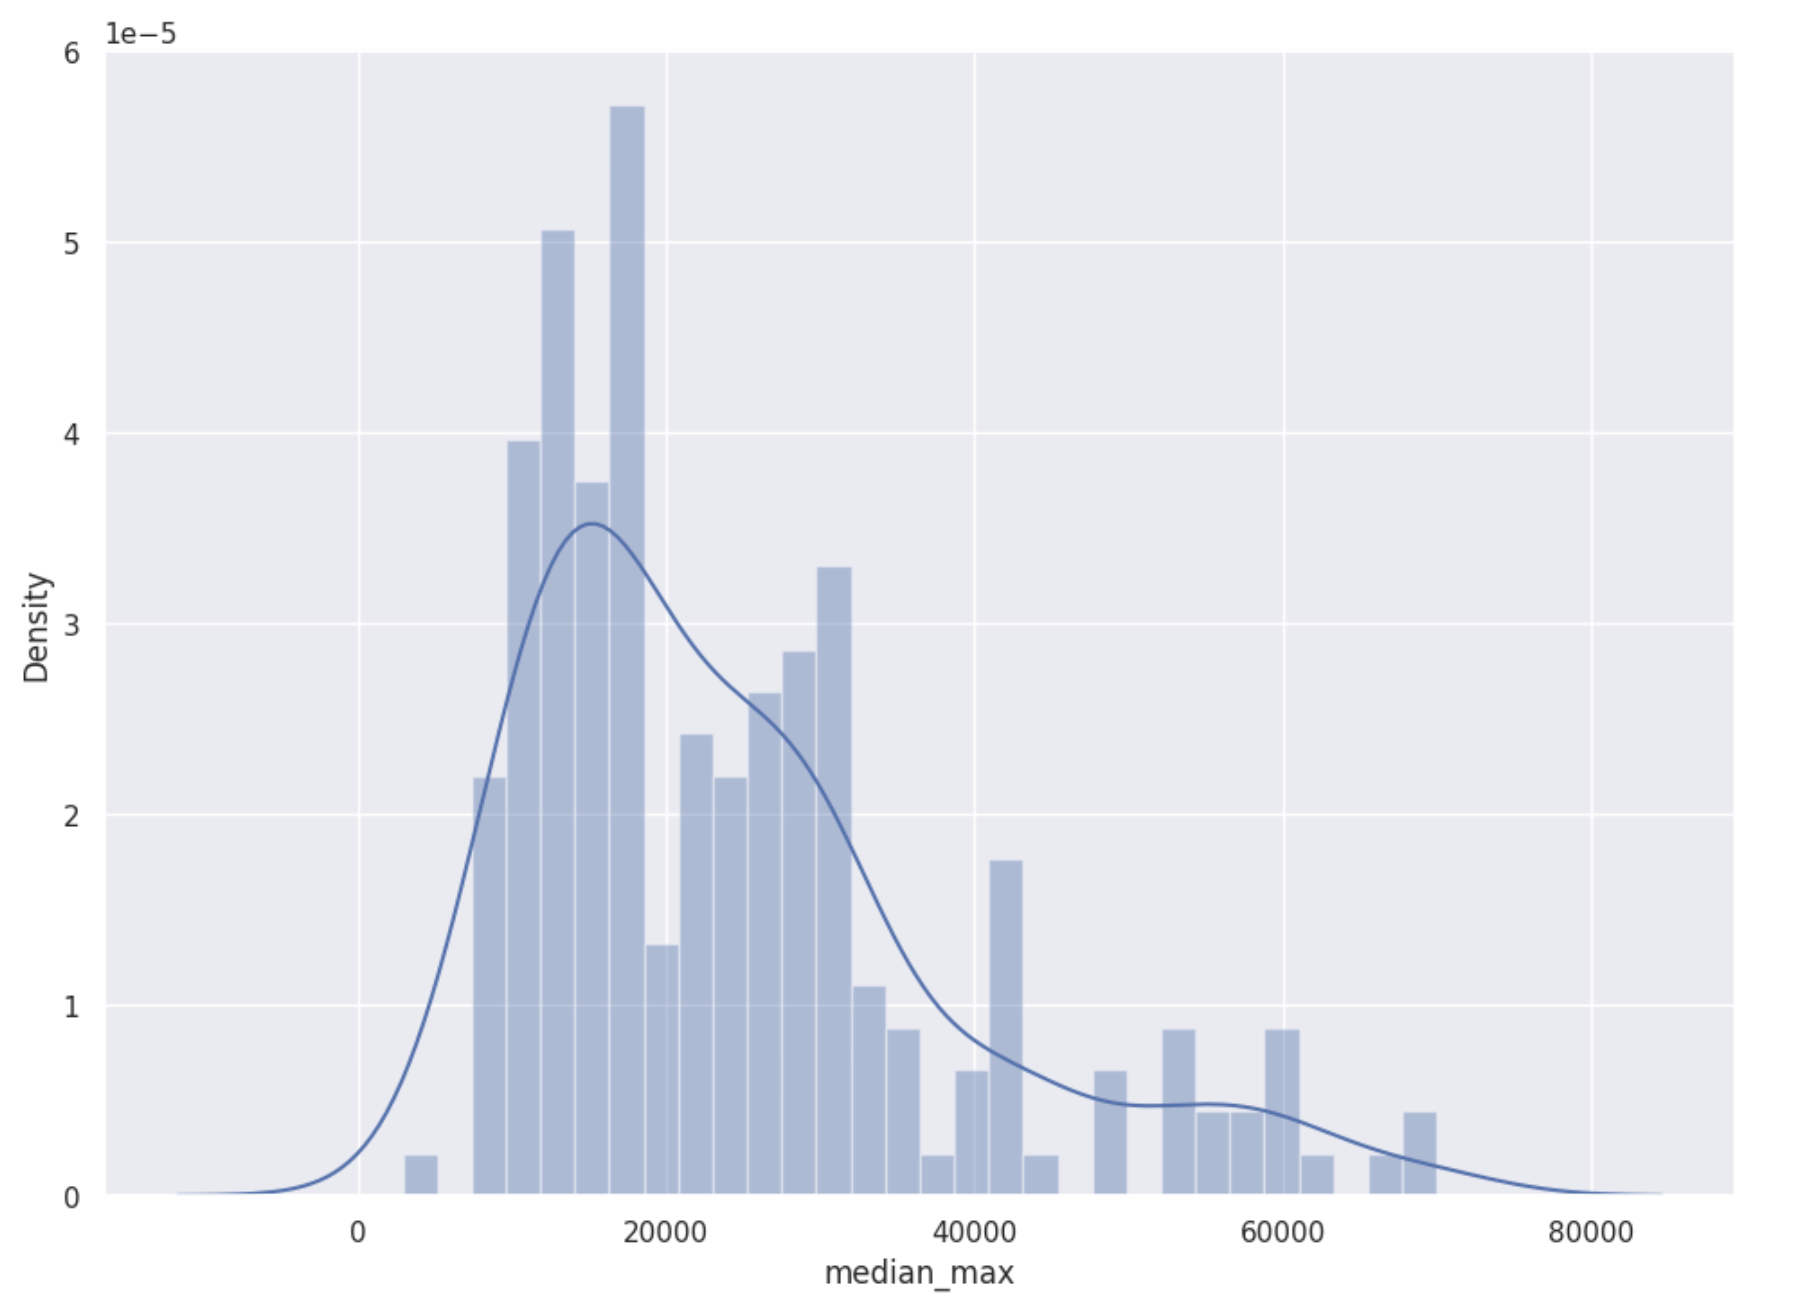
\includegraphics[width=0.6\textwidth, center]{verteilung_max.png}
    \caption[Verteilung von dem Preis Features \emph{median\_max}]{Verteilung von dem Preis Features \emph{median\_max}}
    \label{img:verteilung_max}
\end{figure}

Anders als bei dem Minimalen Median Preis, kann bei dem Maximalen Median Preis keine Normalverteilung erkannt werden. Hier wirken die Werte recht verstreut.

\begin{figure}[h]
    \centering
    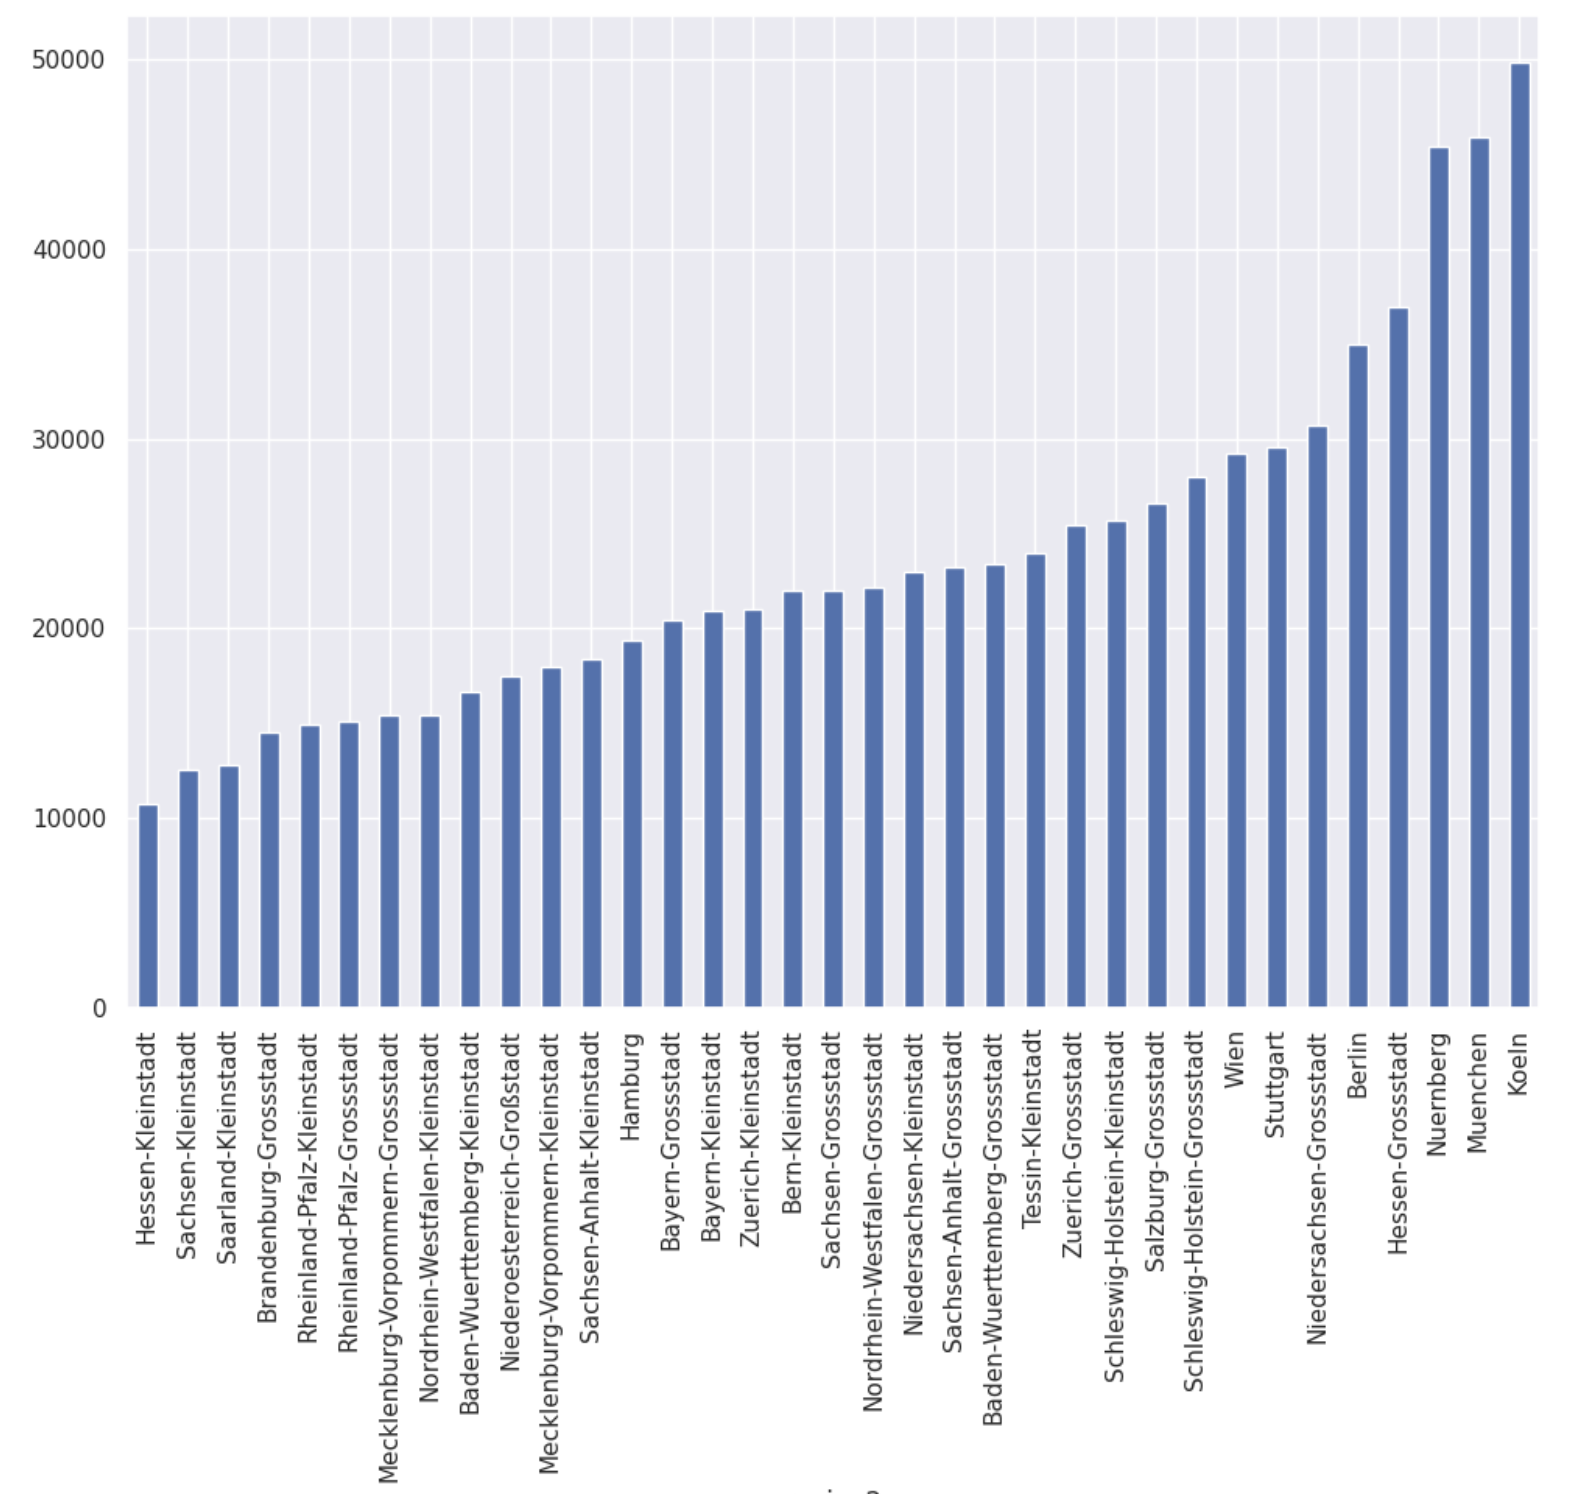
\includegraphics[width=1\textwidth, center]{avg_max_region.png}
    \caption[Durchschnittlicher maximal Preis pro Region]{Durchschnittlicher maximal Preis pro Region}
    \label{img:avg_max_city}
\end{figure}

Abbildung \ref{img:avg_max_city} zeigt, dass es auch deutliche Unterschiede bei den einzelnen Regionen gibt. Eine weitere interessante Erkenntnis ist die, dass es bei dem Maximalen Median Preis eher so ist, dass die Großstädte wie Köln und München eher zu einem höheren Maximalen Preis tendieren.

\subsubsection{Hotelart Feature}
Die Hotelart bildet einen essenziellen Bestandteil, um umfassende Einblicke in die Charakteristiken eines Hotels zu gewinnen. Sie liefert nicht nur Informationen über den Zweck und die Ausrichtung der Unterkunft, sondern ermöglicht auch eine präzise Identifikation der Zielgruppe, die das Hotel anspricht \cite{User.20.01.2024}. Die Zielgruppe eines Hotels ist zudem eine wertvolle Information wenn es darum geht Preise für das Hotel zu gestalten, zumindest ist so die Annahme. Auch in diesem Fall kann wieder nach der Hotelart gruppiert werden und jeweils der Minimale und Maximale durchschnittliche Preis angezeigt werden.

\begin{figure}[h]
    \centering
    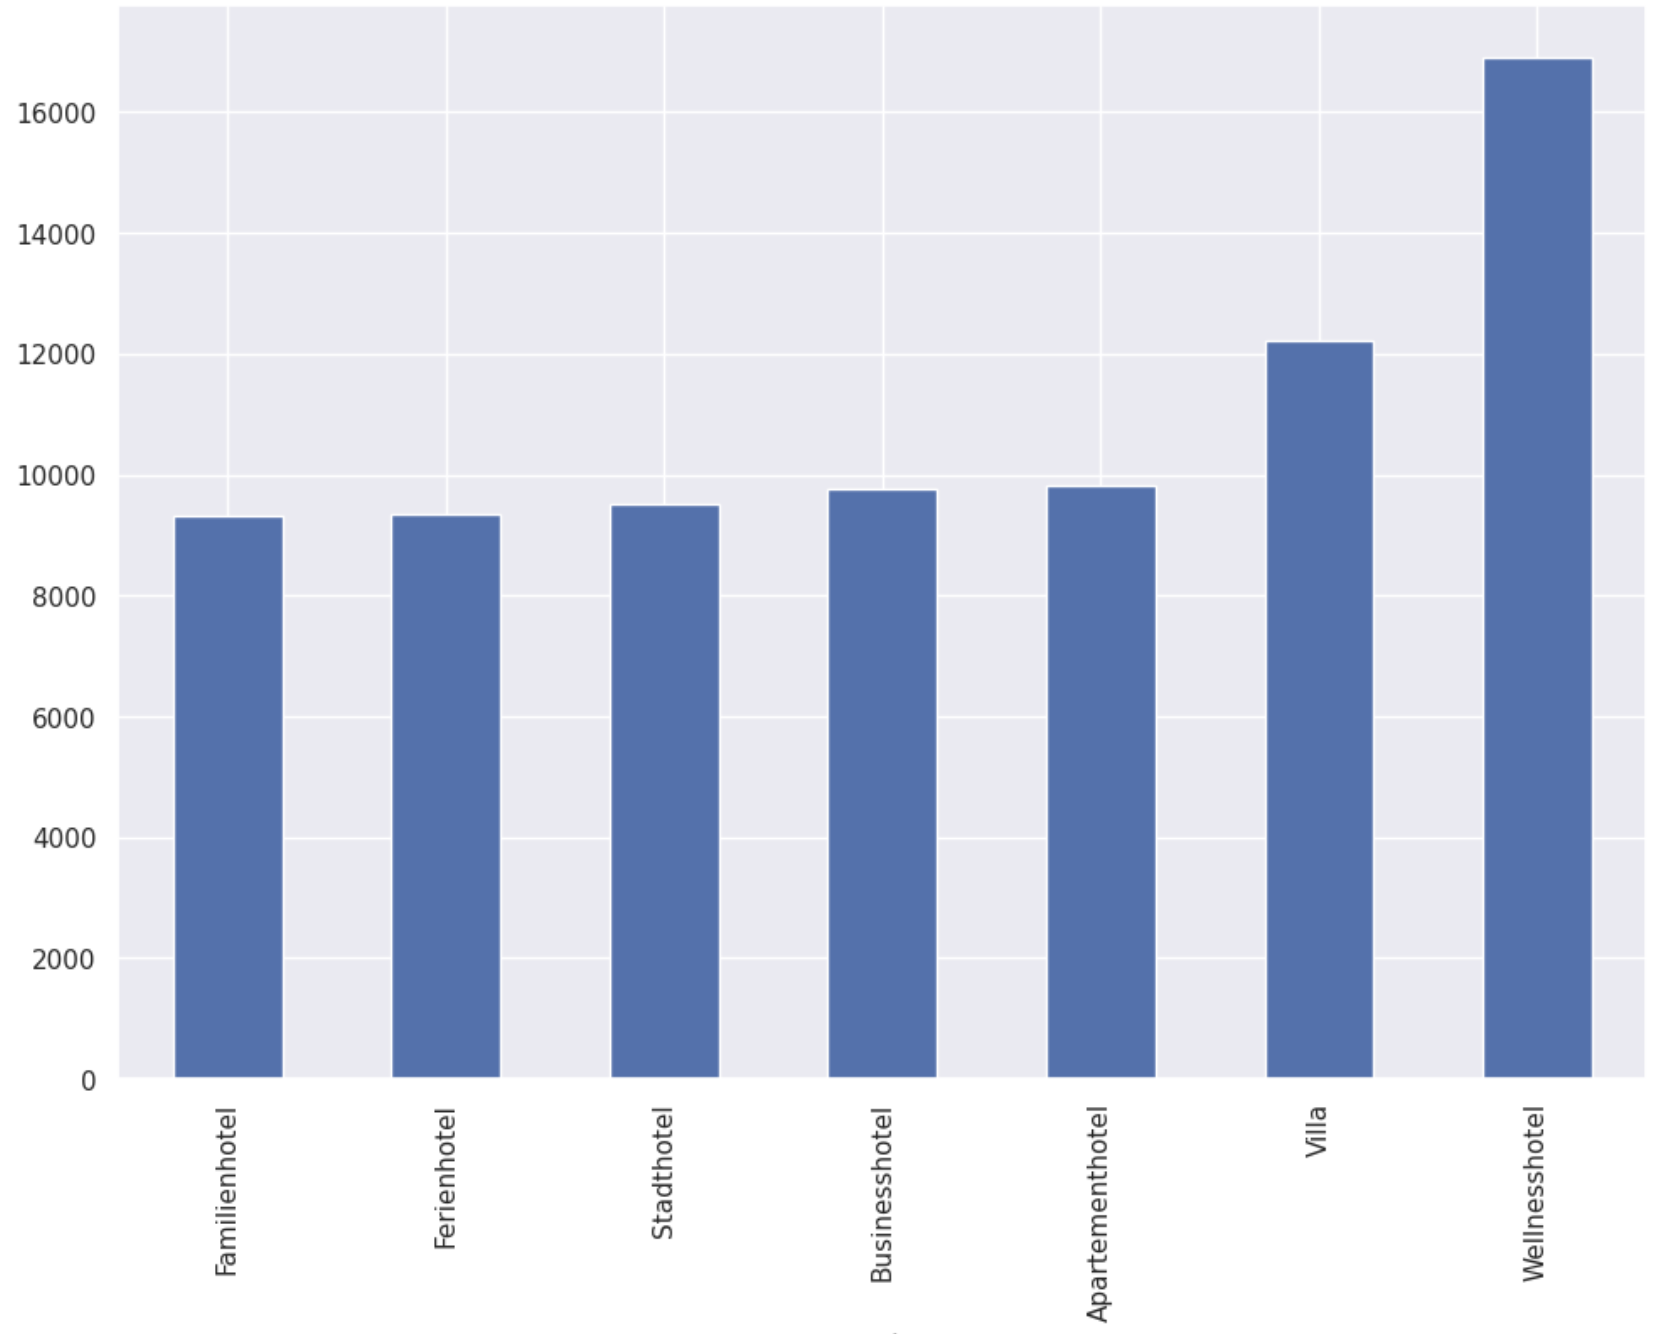
\includegraphics[width=0.6\textwidth, center]{avg_min_art.png}
    \caption[Durchschnittlicher minimal Preis pro Hotelart]{Durchschnittlicher minimal Preis pro Hotelart}
    \label{img:avg_min_art}
\end{figure}

\begin{figure}[h]
    \centering
    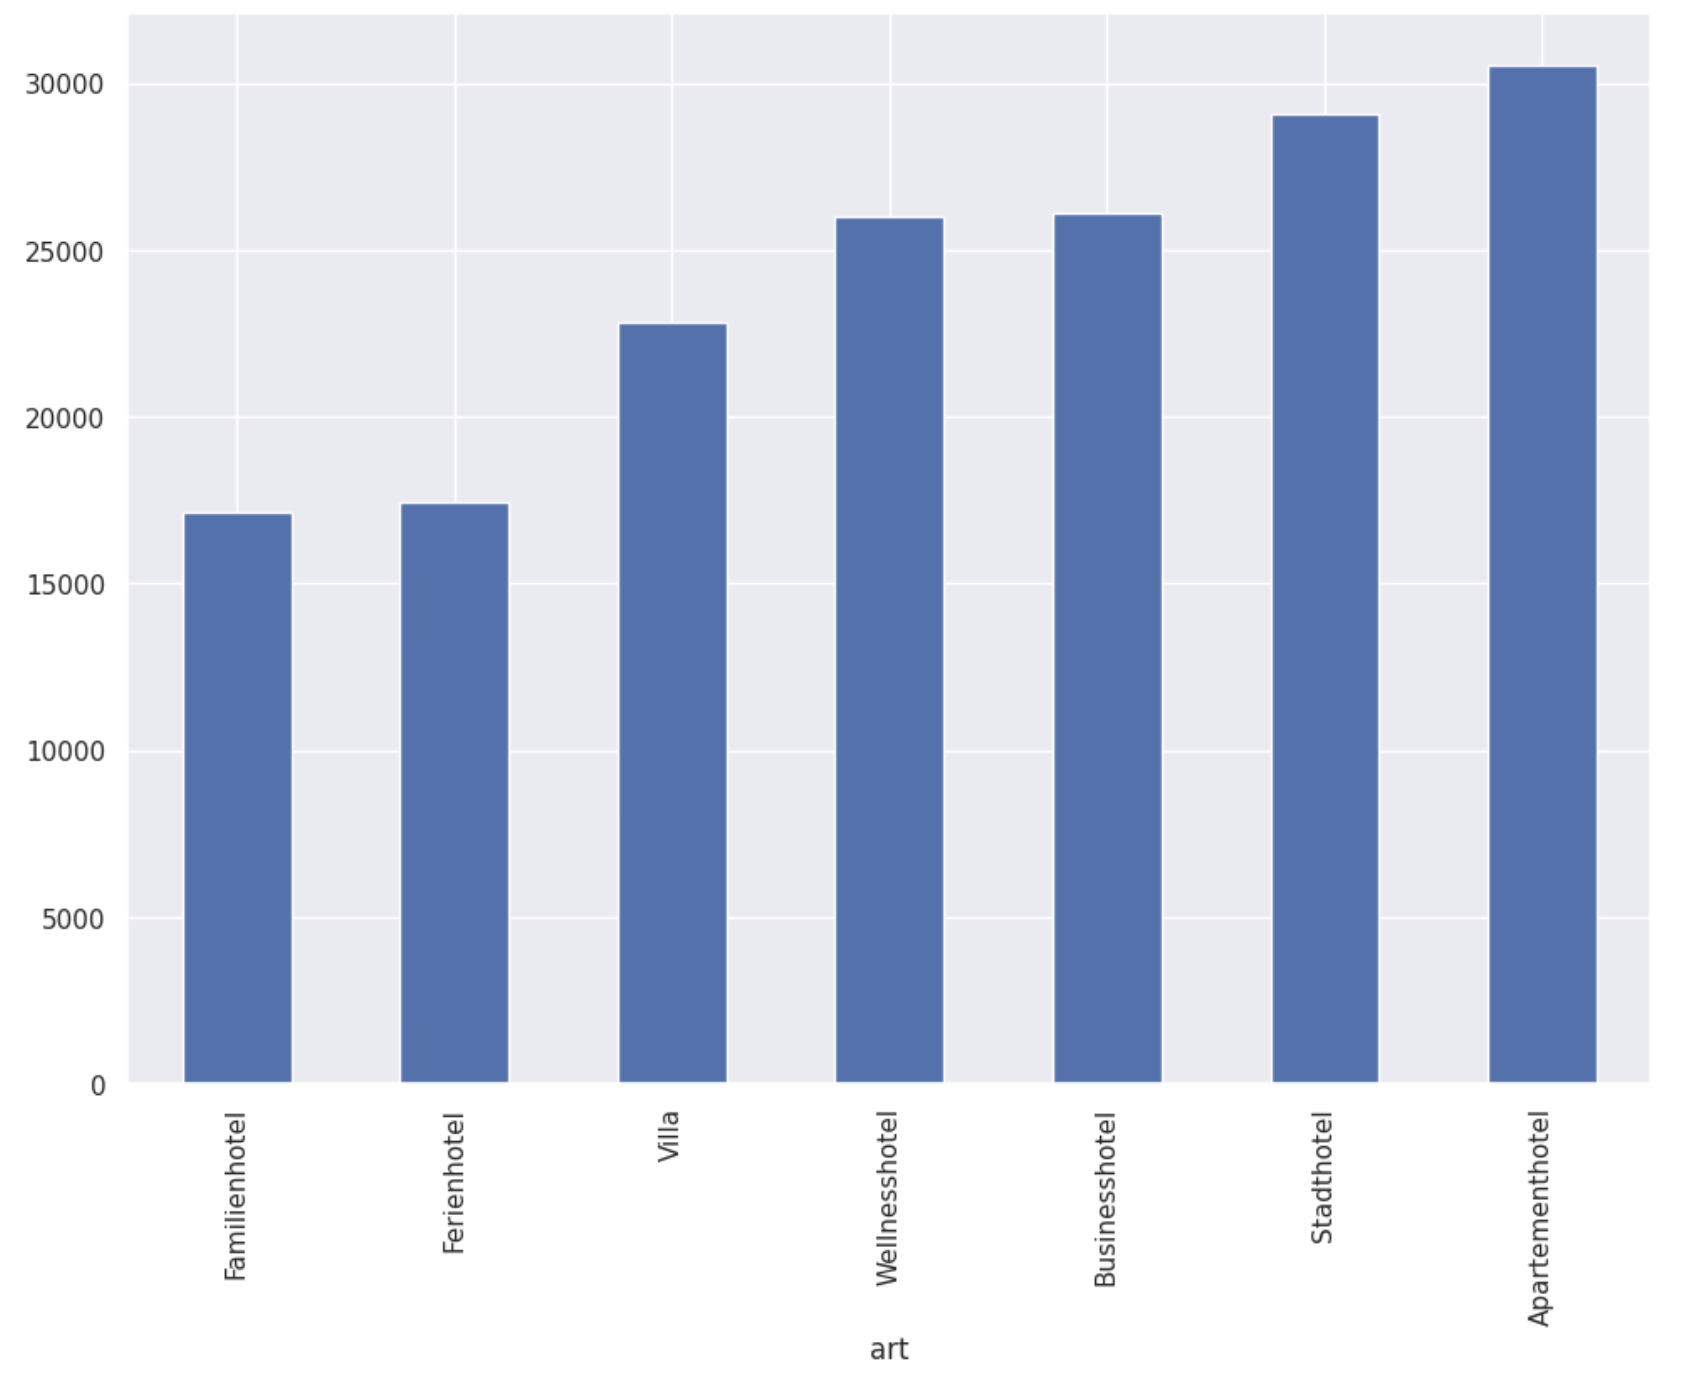
\includegraphics[width=0.6\textwidth, center]{avg_max_art.png}
    \caption[Durchschnittlicher maximal Preis pro Hotelart]{Durchschnittlicher maximal Preis pro Hotelart}
    \label{img:avg_max_art}
\end{figure}

Anhand von den zwei Abbildungen \ref{img:avg_min_art} und \ref{img:avg_max_art} zeigt sich, dass tatsächlich einen unterschied bei den Preisen auf die Hotelart bezogen gibt. Zudem zeigt sich, dass die zwei Hotelarten \emph{Ferienhotel} und \emph{Familienhotel} in beiden Fällen die gleiche Information wiedergibt und somit auch zu \emph{Ferienhotel} zusammengefasst werden kann. Zudem könnten anhand von \emph{median\_min} noch weitere Hotelarten zusammengefasst werden, jedoch wenn beide Informationen zusammen betrachtet werden, so bleibt es lediglich bei \emph{Ferienhotel} und \emph{Familienhotel}.

\subsubsection{Zimmer Features}
Die letzten zwei Features innerhalb des Datensatzes sind die Features \emph{area\_count} und \emph{areatype\_count} welche die Größe des jeweiligen Hotels repräsentieren. Die Frage die sich hier also stellt ist, ob das Preisverhältnis in irgendeiner Art mit der Größe des Hotels zusammenhängen kann. Hierzu soll zunächst auch erstmal die Verteilung der Zimmeranzahl angeschaut werden:

\begin{figure}[h]
    \centering
    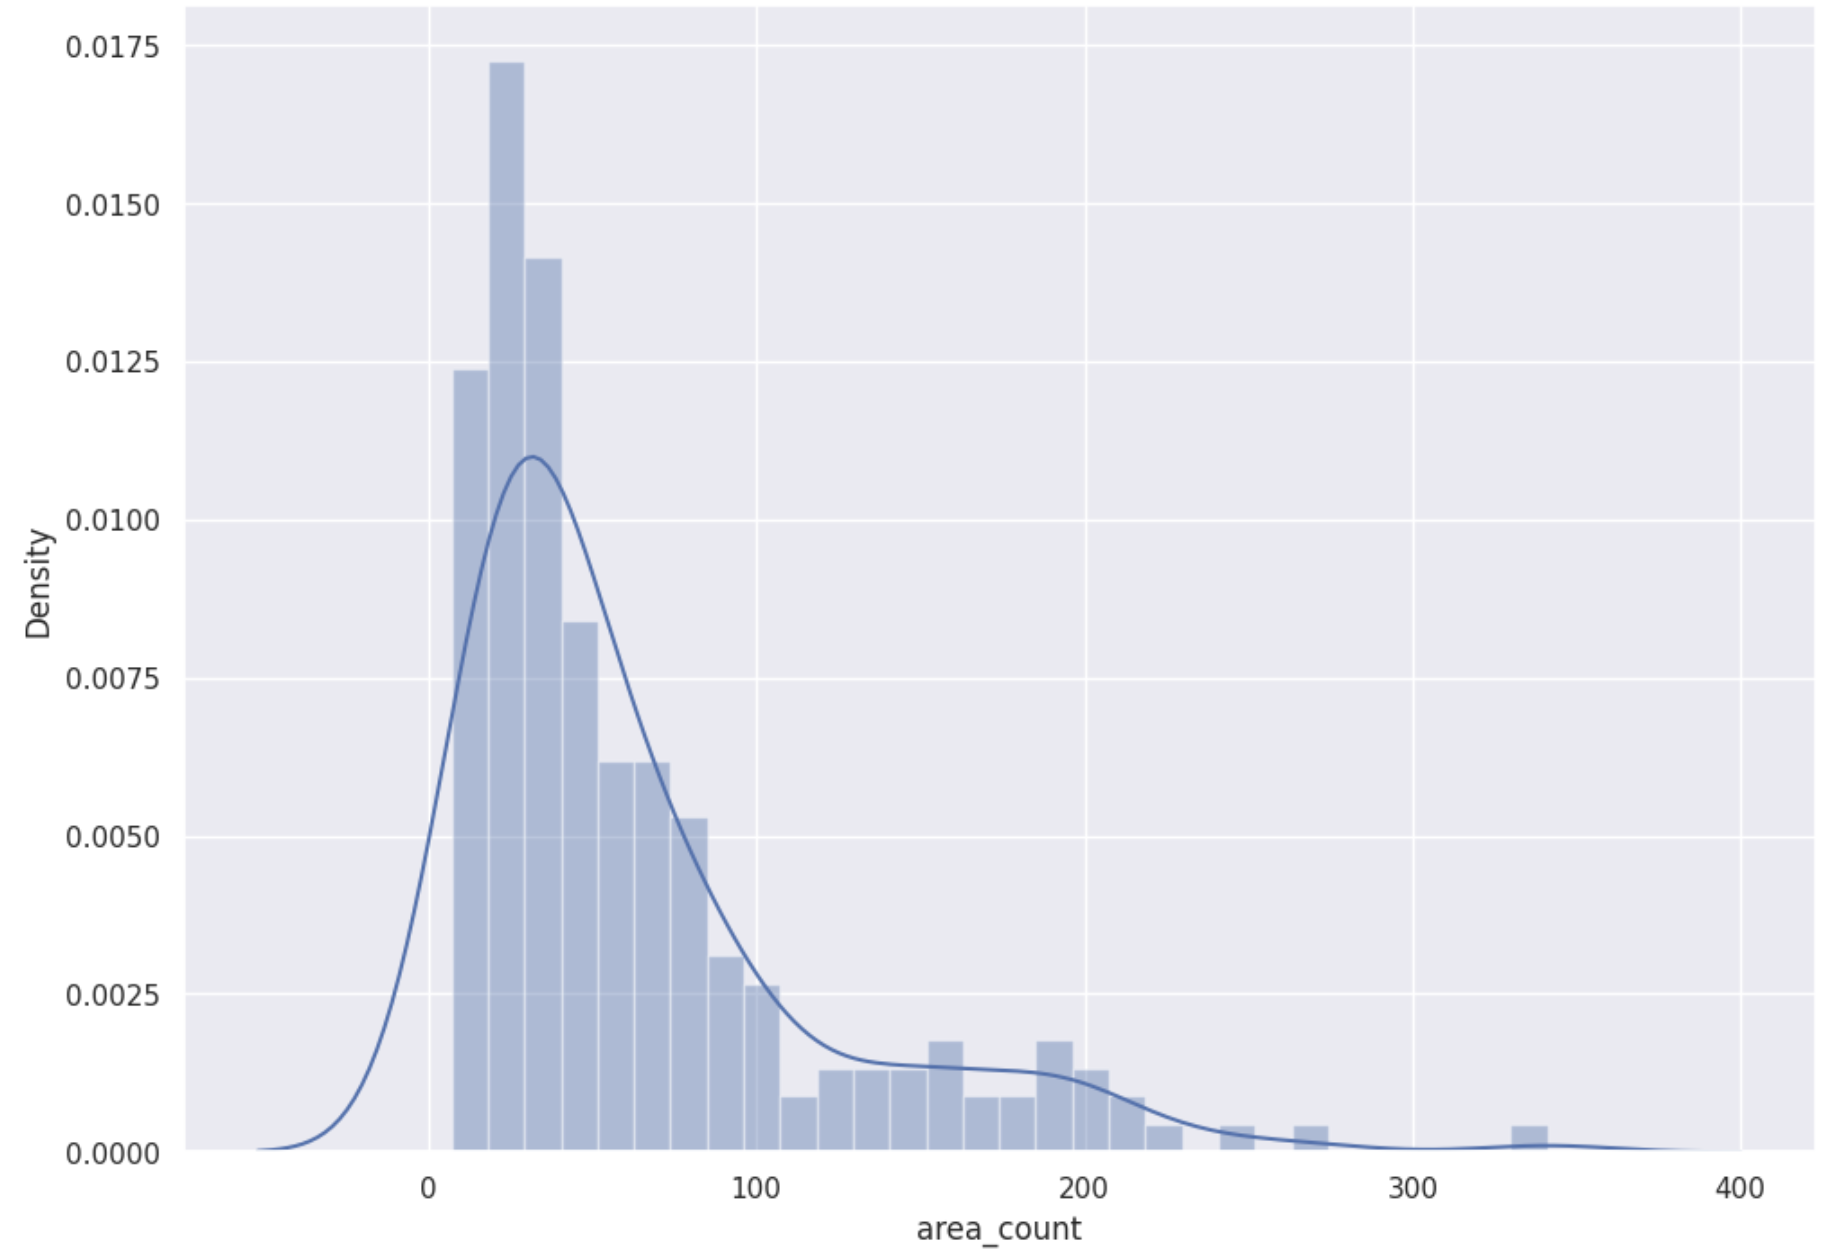
\includegraphics[width=0.6\textwidth, center]{verteilung_area_count.png}
    \caption[Verteilung nach Zimmeranzahl]{Verteilung nach Zimmeranzahl}
    \label{img:verteilung_area_count}
\end{figure}

Die Verteilung zeigt, dass auch recht ausgeprägt ist und nur im Ansatz einer Normalverteilung gleicht. Des Weiteren soll nach der Anzahl der Zimmer gruppiert werden um zu überprüfen wie oft jeder Anzahl vorkommt:

\begin{figure}[h]
    \centering
    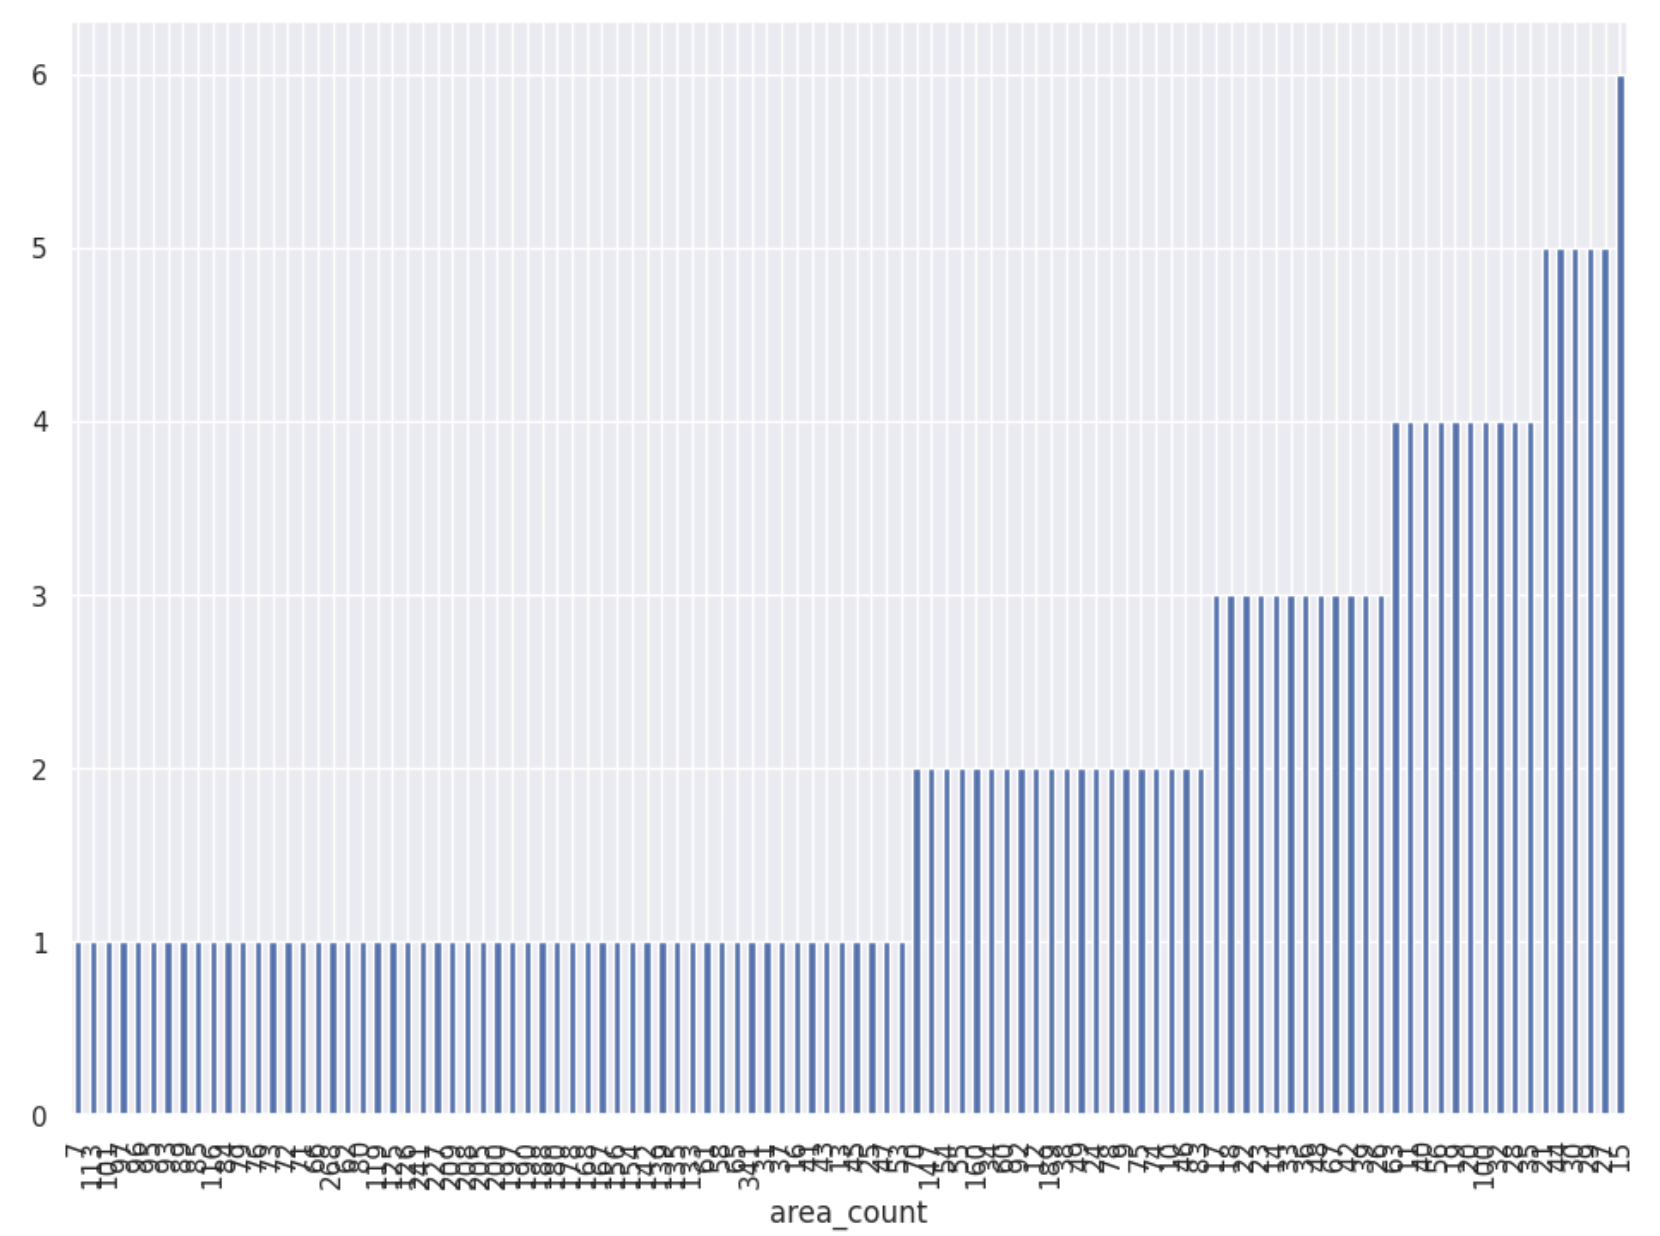
\includegraphics[width=0.6\textwidth, center]{group_area_count.png}
    \caption[Häufigkeit der Zimmeranzahl im Datensatz]{Häufigkeit der Zimmeranzahl im Datensatz}
    \label{img:haufigkeit_area_count}
\end{figure}
Abbildung \ref{img:haufigkeit_area_count} hat gezeigt, dass das Feature \emph{area\_count} zu ausgeprägt ist. Aufgrund dessen, dass das Feature zu ausgeprägt ist und keine Idee vorhanden ist, wie dieses Feature umformuliert werden könnte, wurde beschlossen \emph{area\_count} und \emph{areatype\_count} aus dem Datensatz zu entfernen.
\newline
\newline
Der finale Datensatz welcher für das Modell benutzt werden soll, sieht wie folgt aus:

\begin{figure}[h]
    \centering
    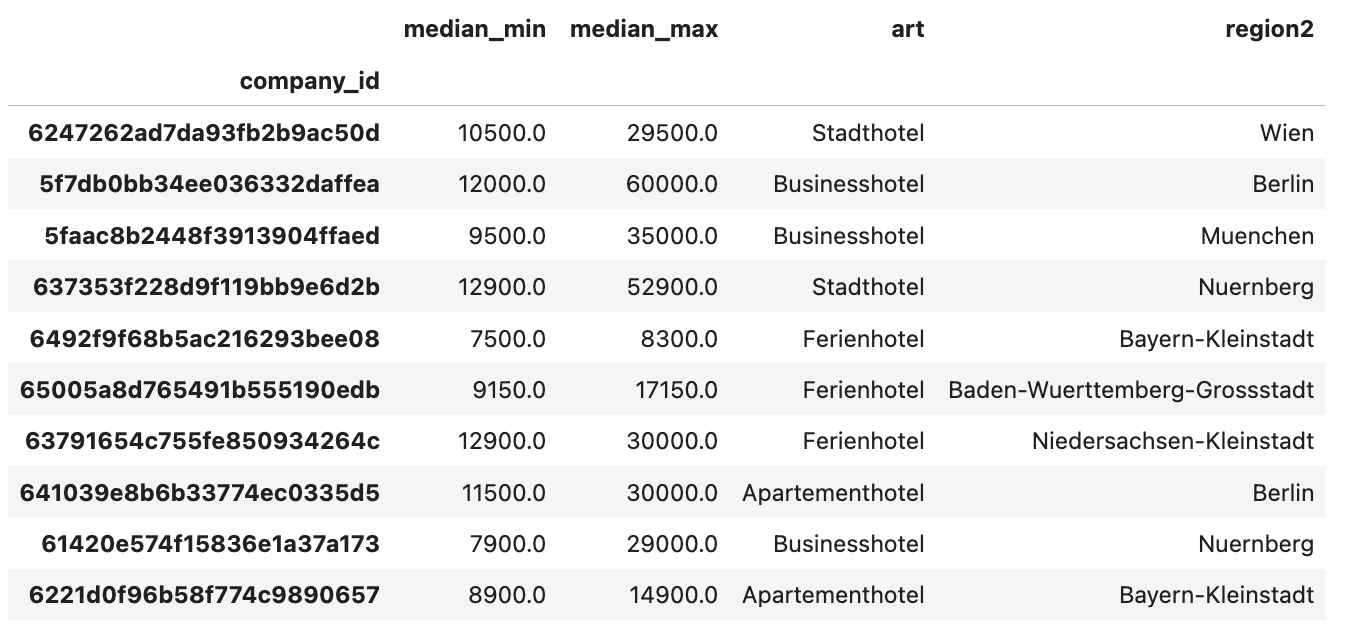
\includegraphics[width=1\textwidth, center]{all_features_4.png}
    \caption[Finaler Datensatz für das Modell]{Finaler Datensatz für das Modell}
    \label{img:all_features_4}
\end{figure}